\documentclass{beamer}
\usetheme{AnnArbor}
\usecolortheme{beaver}
\usepackage{graphicx}
\graphicspath{{images/}}
\usepackage[T1]{fontenc}
\usepackage[utf8x]{inputenc}
\usepackage[french]{babel}
\usepackage{subcaption}
\usepackage{listings} % package pour insérer les codes
\usepackage{xcolor}
\definecolor{codegreen}{rgb}{0,0.6,0} % Définir les couleurs pour les codes
\lstset{frame=tb,
  language=Java,
  aboveskip=3mm,
  belowskip=3mm,
  showstringspaces=false,
  columns=flexible,
  basicstyle={\small\ttfamily},
  numbers=none,
  numberstyle=\tiny\color{gray},
  keywordstyle=\color{blue},
  commentstyle=\color{codegreen},
  stringstyle=\color{black},
  breaklines=true,
  breakatwhitespace=true,
  tabsize=3
}

\usepackage{mathtools} % Pour les symbols mathématiques



  
\newenvironment<>{shortblock}[2]{.5\textwidth}{
    \setlength{\textwidth}{##1}
    \begin{actionenv}##3
        \def\insertblocktitle{##2}
        \par
        \usebeamertemplate{block begin}
        \par
        \usebeamertemplate{block end}
    \end{actionenv}
}

\title[Soutenance de fin d'études]{Automatisation de Tests fonctionnels}

\author{Qilin ZHANG}
\institute{Sorbonne Université - Master 2 Informatique STL Alternance}
\date{5 Septembre 2019}
\subject{presentation}

% Table des matières à chaque début de section
\AtBeginSubsection[]
{
  \begin{frame}
    \frametitle{Plan}
    \tableofcontents[currentsection, currentsubsection]
  \end{frame}
}
\begin{document}
    % page de titre
    \begin{frame}
        \titlegraphic{
            
\includegraphics[width=2cm]{Logo_officiel_Sorbonne_University}\hspace*{1.75cm}~%
            
\includegraphics[width=2cm]{SAP_R_grad}
        }
        
        \titlepage
        \footnotesize Tuteur d'entreprise: Camilla CHRISTIANSEN, Sébastien COUDRAY \\
Tuteur universitaire: Emmanuel CHAILLOUX, Binh-Minh BUI-XUAN
    \end{frame}
    
    % Logo 
    \logo{
            
\includegraphics[height=0.5cm]{Logo_officiel_Sorbonne_University}
            
\includegraphics[height=0.5cm]{SAP_R_grad}
        }
        
    % plan
    \begin{frame}
        \frametitle{Plan}
        \tableofcontents
    \end{frame}
    
    \section{Présentation de l'entreprise et de l'équipe}
        \subsection{Présentation de SAP}
        
        %%%%%% Frame 1 %%%%%%
        \begin{frame}[t]
            \begin{block} {Historique de SAP}
                SAP SE (Systems, Applications \& Products in Data Processing), fondé par 5 anciens employés d'IBM en 1972
            \end{block}
            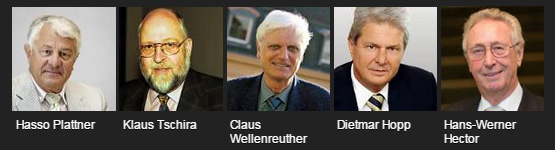
\includegraphics[width=5cm,]{sap_founders.jpg}
            \begin{block}{SAP en 3 points}
            \begin{itemize}
                \item 1\textsuperscript{er} éditeur de logiciels en Europe et 4\textsuperscript{ème} dans le monde
                \item Le plus grand fournisseur mondial de logiciels d’application d’entreprise
                \item Entreprise internationale : 98000 employés répartis dans 147 pays et 437000 clients de 180 pays.
                
            \end{itemize}
            \end{block}
            
\includegraphics[width=0.3\textwidth]{SAP_Best_R_grad_blk.jpg}
        \end{frame}
       
       
        
        \subsection{Mon rôle au sein de l'équipe}
        %%%%%% Frame 6 %%%%%%
        \begin{frame}[t]
        \frametitle{Mon rôle au sein de l'équipe P\&I LoB Finance}
            \begin{block}{Equipe}
                \begin{itemize}
                    \item Apprenti Ingénieur Qualité intégré au sein de  l'équipe P\&I S/4HANA LoB Finance France. Elle est composée d'une quarantaine de personnes qui utilisent SCRUM comme méthode de travail.
                    \item Développement et maintenance de SAP Financial Consolidation (FC), une application de consolidation financière et de reporting de gestion développée depuis 1999.
                \end{itemize}
            \end{block}
        \end{frame}
    
        \begin{frame}{Mon rôle au sein de l'équipe P\&I LoB Finance}
            \begin{block}{Mon rôle}
                \begin{itemize}
                    \item Automatiser des scénarios de tests fonctionnels et tests de non-régression pour le client FC Web HTML5.
                \end{itemize}
            \end{block}
            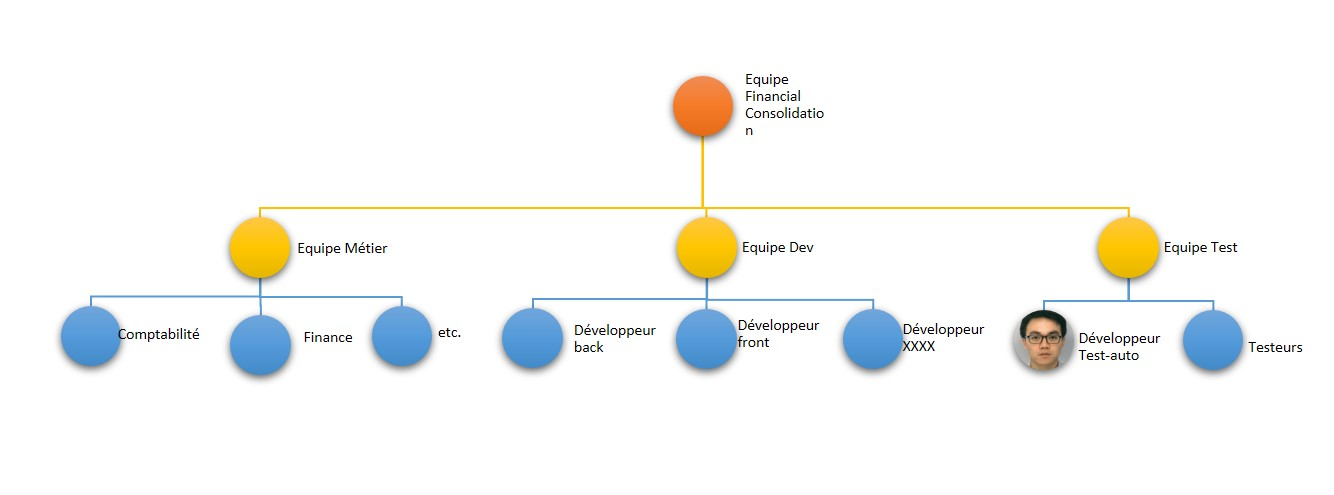
\includegraphics[width=12cm]{role_organisation.jpg}
        \end{frame}
        
    \section{Contexte et problématique}

        
        %%%%%% Frame 9 %%%%%%
        \subsection{Test de nouvelles fonctionnalités et test de non-régression}
        %%%%%% Frame 10 %%%%%%
        \begin{frame}[t]
            \frametitle{Deux types de test}
            \begin{block}{Test des nouvelles fonctionnalités}
                Test fonctionnel sur les nouvelles fonctionnalités implémentés lors du dernier sprint.
            \end{block}
            
            \begin{block}{Test de non-régression}
            Le but de la non-régression est de s'assurer qu'après une correction de bug, de nouveaux bug n'ont pas été introduits ou découverts dans l'application. \newline
            \textcolor{orange}{Ces tests durent tout au long du développement du produit, d'où l'intérêt de les automatiser pour libérer du temps de test manuel sur les nouvelles fonctionnalités.}
            \end{block}
            \pause
            %\begin{alertblock}{{\LARGE{Ces deux test assurent la qualité du produit}}}
            
            %\end{alertblock}
            \centering
            \alert{{\Large{\textbf{Ces deux types de test assurent la qualité de produit !!!}}}}
        \end{frame}
        
        \subsection{Test d'impression}
        
        %%%%%% Frame 11 %%%%%%
        \begin{frame}
            \frametitle{Problématique du test d'impression}
            \begin{itemize}
                \item FC contient une fonctionnalité d'impression des rapports, ces rapports sont au format PDF, le \textit{\textbf{test de non-régression}} doit assurer la qualité de cette fonctionnalité.
                \pause
                \item Vérifier si l'impression de différentes versions de rapports donnent les mêmes résultats, et le test doit indiquer les différences s'il en trouve.
            \end{itemize}
             
            \begin{figure}[H]
                \centering
                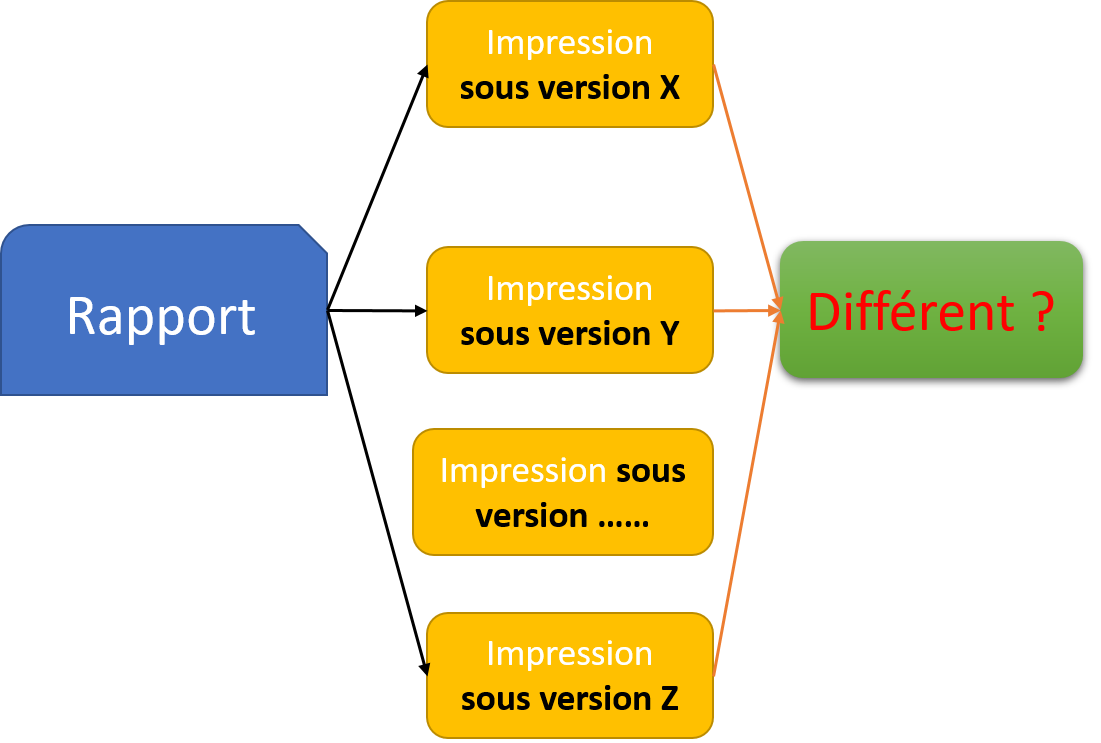
\includegraphics[width=7cm]{problematique_print.png}
                \label{fig:problem_print}
            \end{figure}
                
        \end{frame}
        
        %%%%%% Frame 12 %%%%%%
        \begin{frame}[t]
            \frametitle{Etat de travail}
            \begin{block}{Etat des tests d'impression avant mon arrivée}
                \begin{itemize}
                    \item Avant mon arrivée, l'équipe faisait ces tests manuellement. L'exécution répétée de ces scénarios entraînait un risque d'erreur humaine important dans la comparaison des fichiers PDF ainsi qu'une perte de temps, d'où le besoin d'automatiser ces tests.
                    \item Le projet de Test-Auto utilisant le langage Java et plusieurs autres technologies a été développé depuis quelques années, et il continue à couvrir de plus en plus de fonctionnalités du produit.
                \end{itemize}
            \end{block}
        \end{frame}
        
        \begin{frame}[t]{Etat de travail}
            \begin{block}{Statut des autres équipes de SAP France}
                \begin{itemize}
                    \item Une autre équipe a travaillé sur un projet de comparaison entre deux fichier PDFs pixel par pixel en Java. Ils utilisent la bibliothèque \textit{ice-pdf}, qui génère une image indiquant la différence entre les deux fichiers comparés.
                    \item Cette solution ayant fait ces preuves, nous avons décidé de la récupérer et de l'adapter à nos besoin pour notre projet Test-Auto.
                \end{itemize}
            \end{block}
        \end{frame}
    
        
    \section{Travaux réalisés}
        \subsection{Architecture du projet Test-Auto}
        %%%%%% Frame 14 %%%%%%
        \begin{frame}[t]
            \frametitle{Projet Test-Auto : Comment ça marche ?}
            \begin{itemize}
                \item Projet Test-Auto est un projet configuré par Jenkins et plusieurs types de machines virtuelles : 
                    \begin{enumerate}
                        \item \textbf{VM de Jenkins serveur:} Contient toutes les configurations de Jenkins pour le projet Test-Auto.
                        \item \textbf{VM du DB de FC: } La DB de FC: SAP HANA, Oracle 12, Microsoft SQL Server.
                        \item \textbf{VM de ressources:} Contient toutes les ressources que les test automatisé a besoin.
                        \item \textbf{VM du DB de Reporting:} La DB sauvegarde les logs de tests, et visualiser ces logs au rapport Excel.
                        \item \textbf{VM de Test:} L'environnement de test avec les logiciels et bibliothèques installés: Windows, Jenkins slave, Maven, FC client, IE, Chrom, Firefox.
                    \end{enumerate} 
            \end{itemize}
        \end{frame}
        
        \begin{frame}[t]
            \frametitle{Projet Test-Auto : Comment ça marche ?}
            \begin{block}{La procédure d'un test automatisé}
                \begin{enumerate}
                    \item Jenkins déclenche la restauration de DB de FC sur la VM de Test
                    \item Jenkins déclenche la récupération des ressources de la VM de ressources
                    \item Jenkins déclenche le test sur la VM de Test
                    \item Jenkins déclenche la remontée des résultats de test dans la DB de Reporting
                \end{enumerate}
            \end{block}
        \end{frame}
        
        \begin{frame}{Projet Test-Auto : Comment ça marche ?}
            \centering
            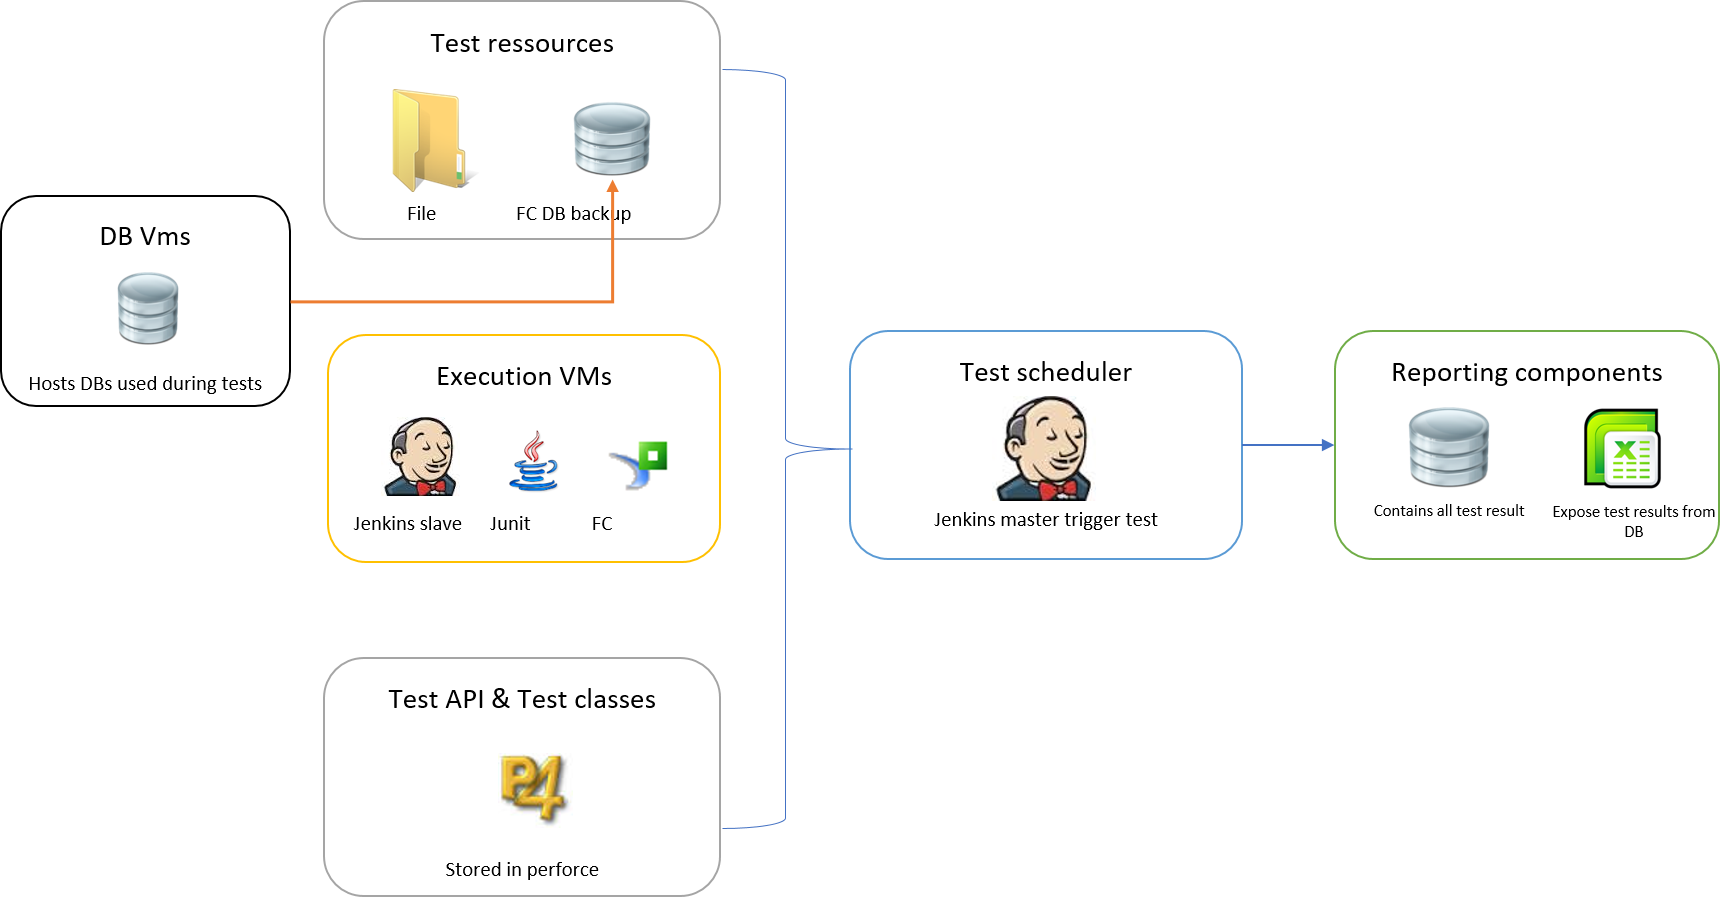
\includegraphics[width=10cm]{TestAuto_architecture.png}
        \end{frame}
        
        \subsection{Développements réalisés}
        %%%%%% Frame 15 %%%%%%
        \begin{frame}[t]
            \frametitle{Automatisation des scénarios de test avec Silktest}
            \begin{block}{Contenus de la tâche}
                \begin{itemize}
                    \item Lire et comprendre le code existant du projet Test-Auto.
                    \item Implémentions de nouveaux scénarios de test en utilisant les technologies déjà misent en place pour le projet Test-Auto: Silktest (Silk4J), Junit, Maven, Jenkins.
                \end{itemize}
            \end{block}
            
            \pause
            \begin{block}{Résultats des premières tâches effectués}
                \begin{enumerate}
                        \item Bonne compréhension de l'architecture des Test-auto
                        \item Apprentissage du développement avec Silktest: 
                            \begin{itemize}
                                \item Comment Silktest interagi avec les contrôles de l'application en écrivant des requêtes XPath.
                            \end{itemize}
                    \end{enumerate}
            \end{block}
        \end{frame}
        
        %%%%%% Frame 16 %%%%%%
        \begin{frame}
            \frametitle{Comparaison entre deux PDF}
            \begin{columns}
            \column{0.7\textwidth}
            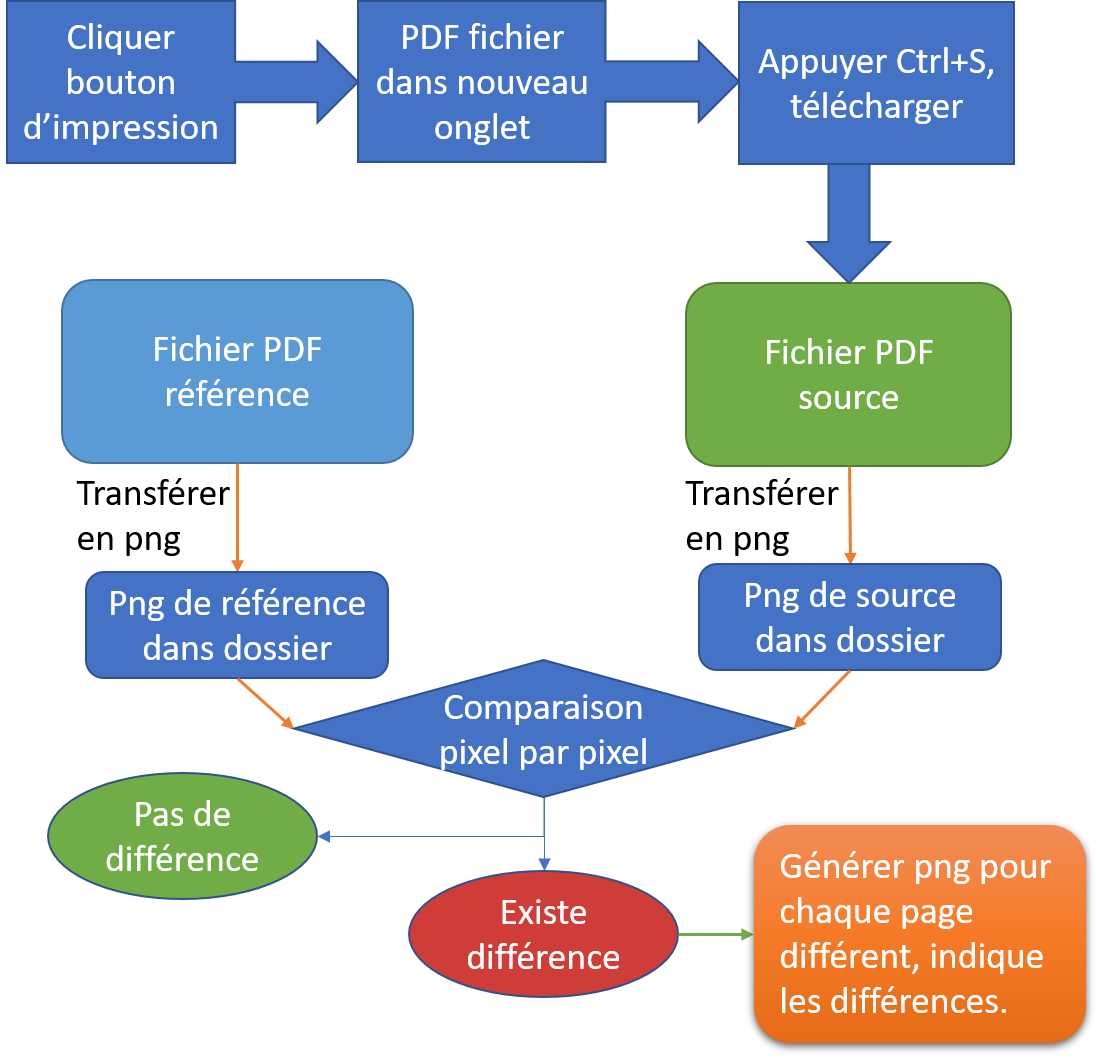
\includegraphics[width=8cm]{process_compar_pdf.png}
            \column{0.3\textwidth}
            \textcolor{red}{\textbf{Résulat : \newline \newline}}
            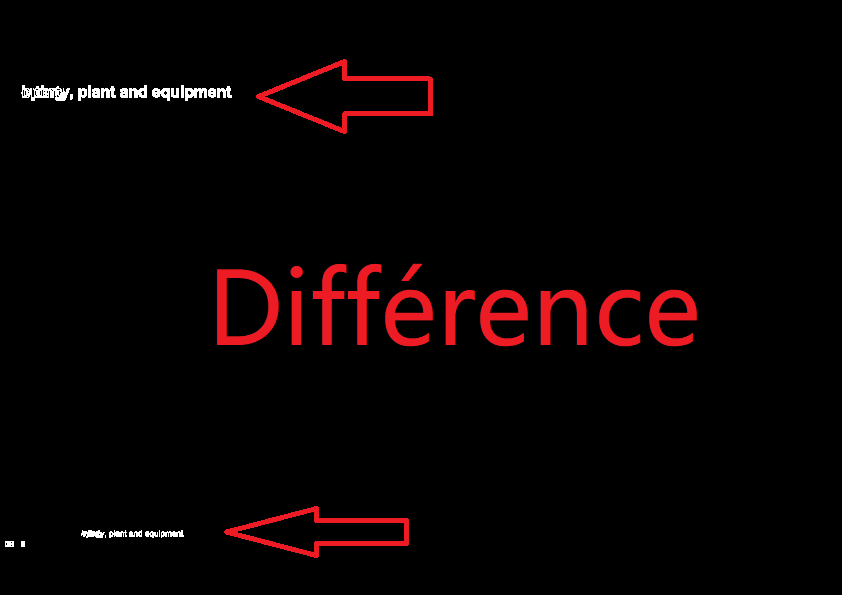
\includegraphics[width=\textwidth]{png_difference.png}
            \end{columns}
        \end{frame}
        
        
        
        \begin{frame}[t]{Comparaison entre deux PDF}
            \begin{block}{Résultat}
                \begin{itemize}
                    \item Les erreurs de test sont affichés dans les logs de test
                        \begin{enumerate}
                            \item Dans l'image de gauche, "OK" désigne un test qui passe bien et "ERROR" veut dire qu'il y a une différence dans le rapport.
                            \item Dans l'image de droite on voit les différences entre les rapports.
                        \end{enumerate}
                \end{itemize}
            \end{block}
            \begin{columns}
                \column{0.5\textwidth}
                \begin{figure}
                    \centering
                    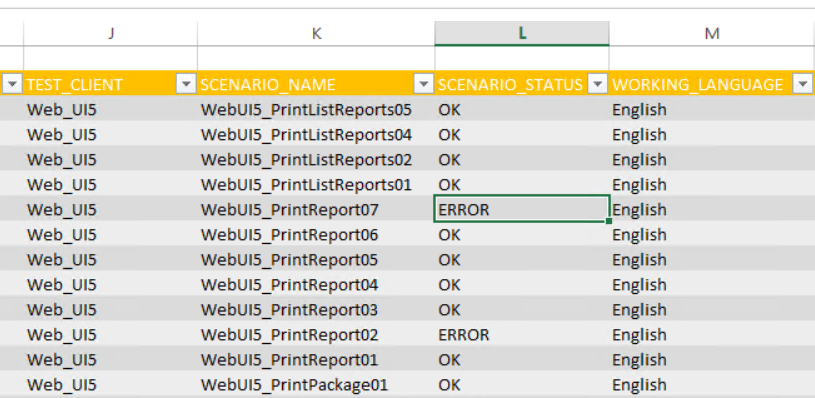
\includegraphics[height=2.65cm]{test_result.PNG}
                    \caption{Résultat de test}
                    \label{fig:result_test_label}
                \end{figure}
                
                \column{0.5\textwidth}
                \begin{figure}
                    \centering
                    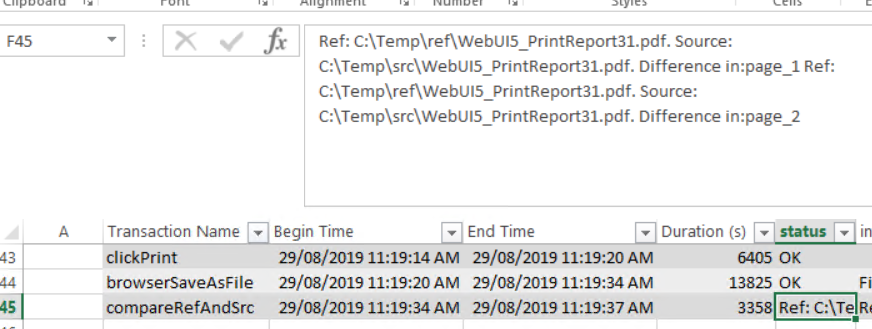
\includegraphics[height=2.3cm]{test_error_detail.PNG}
                    \caption{Détaille d'une erreur}
                    \label{fig:result_error_detail_label}
                \end{figure}
            \end{columns}
        \end{frame}
        
        %%%%%% Frame 17 %%%%%%
        \begin{frame}
        \frametitle{Téléchargement de zip, unzip, comparaison de PDF}
            \begin{block}{Problématique}
                \begin{itemize}
                    \item Pour certains scénario de tests nous avons besoin de télécharger un fichier zip.
                    \item Le suffix du nom de ce zip contient un GUID\textit{(globally unique identifier)}. 
                    \item Ce zip contient un nombre connu de fichiers au format pdf qui ont tous le même GUID comme préfixe.
                \end{itemize}
            \end{block}
            \pause
            \begin{block}{Solution}
                \begin{itemize}
                    \item Utilisation de la bibliothèque \textit{java.util.zip.ZipEntry} et \textit{java.util.zip.ZipInputStream} afin de décompresser le zip.
                    \item Triage des fichiers par date de créations puis renommage des noms par ceux défini dans les scénarios. Pour trier, j'utilise les $\lambda$-Expression.
                    \item Comparaison des fichiers avec les références. 
                \end{itemize}
            \end{block}
        \end{frame}
        
         %%%%%% Frame 18 %%%%%%
        \begin{frame}[t]
            \frametitle{Comparaison de deux répertoire avec $\lambda$-Expression}
            \begin{block}{Problématique}
                \begin{itemize}
                    \item Téléchargement d'un fichier zip
                    \item Nom des fichiers PDF inconnus, ainsi que leur nombre dans ce zip.
                    \item Autrement dit, nous devons comparer le contenu des deux zip (ils ont le même nombre des PDFs, les PDFs ont les mêmes noms).
                \end{itemize}
            \end{block}
        \end{frame}
        
        \begin{frame}[t]
            \frametitle{Comparaison de deux répertoire avec $\lambda$-Expression}
            \begin{block}{Solution $\lambda$-Expression}
                \begin{enumerate}
                    \item Décompresser le zip téléchargé, et le garder comme répertoire source.
                    \item Parcourir le répertoire de référence et mettre tous les fichiers PDF dans une liste.
                    \item  En prenant chaque élément de cette liste, parcourir le répertoire source, trouver le PDF avec le même nom, puis faire la comparaison en appelant la fonction de comparaison PDF déjà développé.
                    \item Si le nombre de fichier est différent, ou les noms ne sont pas les mêmes, il y aura une Exception Java.
                \end{enumerate}
            \end{block}
        \end{frame}
        
        %%%%%% Frame 19 %%%%%%
        \begin{frame}[fragile] % fragile option est pour insérer les codes
            \begin{block}{Comparaison entre deux répertoire avec $\lambda$-Expression}
            \begin{lstlisting}
Path dirRef = Paths.get(refFolder);
Path dirSrc = Paths.get(srcFolder);
// filter the .pdf file
List<Path> listRefPath = Files.list(dirRef)
	.filter(f -> f.toString().endsWith(".pdf"))
	.collect(Collectors.toList());
for (int ii = 0; ii < listRefPath.size(); ii++){
	Path refPath = listRefPath.get(ii);
	Path srcPath = Files.list(dirSrc).filter(path ->
	    path.getFileName().equals(refPath.getFileName()))
	    .findFirst().get();
	comparePDF(refPath.toString(), srcPath.toString());
}
            \end{lstlisting}
            \end{block}
        \end{frame}
        
        \subsection{Outils et technologies utilisés}
        %%%%%% Frame 20 %%%%%%
        \begin{frame}
        \frametitle{Outils et technologies utilisés}
            \begin{table}[l]
                \centering
                \begin{tabular}{|l|c|c|c|c|}
                    \hline
                    IDE & 
\includegraphics[width=1.6cm]{Eclipse_logo.png} & & &\\
                    \hline
                    Communication &  
\includegraphics[width=1.6cm]{Skype_for_Business_logo.png} & 
\includegraphics[width=1.6cm]{Outlook_logo.png} & & \\
                    \hline
                    Partager & 
\includegraphics[width=1.6cm]{Perforce_Logo.jpg} & 
\includegraphics[width=1.6cm]{OneDriveLogo.png} & 
\includegraphics[width=1.6cm]{OneNoteLogo.png} &\\
                    \hline
                    Outils \& Bibliothèques & 
\includegraphics[width=1.6cm]{junit-logo.png} & 
\includegraphics[width=1.6cm]{Maven_logo.png} & 
\includegraphics[width=1.6cm]{jenkins_logo.png}& 
\includegraphics[width=1.6cm]{silktest_logo.png}  \\
                    \hline
                \end{tabular}
                \label{tab:my_label}
            \end{table}
        \end{frame}
        
    \section{Conclusion}
        %%%%%% Frame 21 %%%%%%
        \begin{frame}[t]
            \begin{alertblock}{Résultats de travail}
                \begin{itemize}
                    \item Les scénarios de test de la première tâches sont bien intégrés dans le projet
                    \item Le projet de test d'impression est bien intégré dans le projet et il fonctionne bien sur le projet Test-auto
                    
                \end{itemize}
            \end{alertblock}
            
            
        \end{frame}
        
        %%%%%% Frame 22 %%%%%%
        \begin{frame}
            \begin{center}
                \LARGE{\textbf{Merci pour votre attention }} \textasciicircum\_\textasciicircum
            \end{center}
            
        \end{frame}
\end{document}